
%----------------------------------------------------------------------------
\section{A probléma bemutatása}
\label{sec:problem}
%----------------------------------------------------------------------------

% Arcfelismerő rendszerek bemutatása (1-1.5 oldal?)
% - hogy működik
% - arc detektálás -> embedding kinyerés -> dataset összevetés
% - egyes részek milyen technológiákat használnak (lehet részletezni kicsit)

% Embedding privacy risk (0.5 oldal?)
% - gdpr problim
% - arclenyomatok rekonstruálhatók
% - biometrics reversible (2019 M george - barrara????)
% - they can carry sensitive information

% - Feladat: hogyan van kódolva a személyes adat az embeddingbe?
% - Feladat: mekkora (?) az embeddingek adatvédelmi kockázata?
% - Feladat: javasoljon védekezési megoldásokat a kockázatok kiszűrésére
% Mit fogok csinálni?
% -> részletek a remarkablen írkálva ide oda

% Arcfelismerő rendszerek bemutatása

Az utóbbi időkben széles körben elterjedt az arcfelismerő rendszerek alkalmazása, mivel az arcfelismerés egy hatékony eszköze a biometrikus azonosításnak. Az modern, gépi tanulás alapú arcfelismerő rendszerek működése több lépésből áll, ezt mutatja be a \ref{fig:fr}. ábra. 

Ahhoz, hogy az arcfelismerő rendszer egy személyt sikeresen azonosítani tudjon kamerafelvétel alapján, először a rendszernek sikeresen meg kell találja az emberi arcokat a képen belül. Az arcok észlelését egy képen arcdetektálásnak nevezzük. Miután sikerült lokalizálni az arcokat, azokat szükséges lehet igazítani képtranszformációk segítségével, hogy úgy tűnjön, mintha az arcokat szemből látnánk. A harmadik lépés, az arc képekből jellemzővektorok (későbbiekben: arclenyomatok) kinyerése, ami leírja az arc főbb vonásait, jellemzőit. Az arclenyomat vektorok összehasonlításával már képes a rendszer összevetni a kameraképen látható személy arcát az adatbázisban tárolt, ismert személyekkel. Ha van találat az adatbázisban, akkor sikeresen be lett azonosítva a személy. \cite{hassan2021face}

\begin{figure}[h]
	\centering
	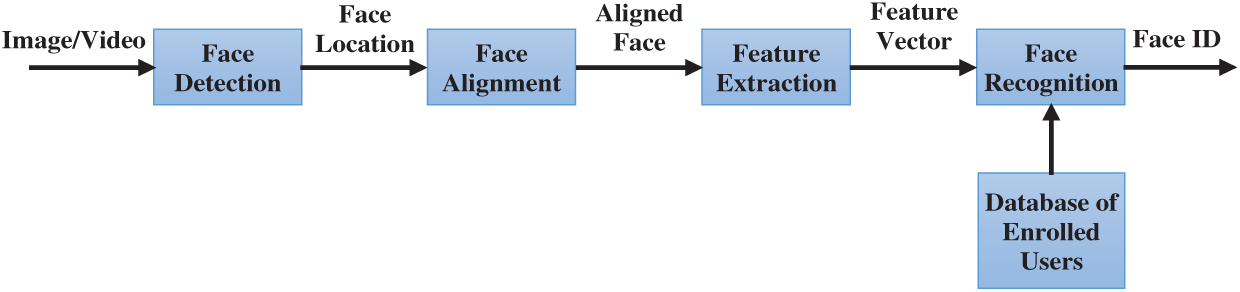
\includegraphics[width=1\columnwidth]{figures/facerecognition.png}
	\caption{Arcfelismerő rendszer folyamatábrája. \cite{hassan2021face}}
	\label{fig:fr}
\end{figure}

Az arcfelismerő rendszerek működésének kifejtése:

\begin{enumerate}
	\item \textbf{Arc detektálása:} Az arcdetektálás az első lépés a sikeres azonosítás érdekében. Itt a cél meghatározni az arcot befoglaló téglalap koordinátáit a képen belül. Ehhez többféle képfeldolgozó módszer is alkalmazott, az egyik a \textit{Haar cascade} alapú módszer, aminek fő előnye a gyors működés, de ennél pontosabb eredmény lehet elérni a \textit{Histogram of Oriented Gradients} (HOG) módszer alkalmazásával. Gyakorlatban, a modern képfeldolgozó szoftvercsomagok mint az OpenCV \cite{opencv_library} tartalmaz arcdetektáló megoldásokat.
	\item \textbf{Arc igazítása:} Miután az arcdetektor segítségével sikerült meghatározni az arcot tartalmazó befoglaló téglalapot, valószínű, hogy az illető nem pont a kamerába néz, valamennyire el van fordulva. Az arc további feldolgozása előtt ezt szükséges képtranszformációs módszerekkel korrigálni. Ehhez előbb mély neurális háló segítségével felismernek az arcon valamennyi kulcspontot (angolul: facial landmark \cite{kazemi2014faciallandmark}). A kulcspontok relatív helyzetéből lehet következtetni, hogy az arcképet milyen irányba, milyen mértékkel szükséges igazítani.
	\item \textbf{Arclenyomat kinyerése:} A következő lépés az arcból egy arclenyomat kinyerése. Ehhez szintén egy mély neurális hálót alkalmaznak, amely a eredeti képből képes jelentősebb kisebb méretű jellemzővektort előállítani, ami tipikusan 128, vagy 512 darab lebegőpontos értékből áll. Azt, hogy az arclenyomatok pontosan az arc mely jellemzőit tartalmazza, azt a \ref{sec:dml}. fejezetben bemutatott mély metrika tanulás alkalmazásával képes megtanulni a neurális háló. Az arclenyomat előnye, hogy jelentősen kisebb méretű az eredeti képnél, mégis alkalmas megkülönböztetés szempontjából jellemezni az emberi arc struktúráját.
	\item \textbf{Arc azonosítása:} Az utolsó lépés az arcról készült arclenyomat összevetése egy adatbázisban tárolt, ismert forrású arclenyomatokkal. Az összevetéshez jellemzően valamilyen távolságmetrikát alkalmaznak, mint a \ref{fig:eukl}. ábrán bemutatott az euklideszi távolságot. Ha megfelelően közeli a két vektor közötti távolság, akkor a képen látható személyt sikerült azonosítania a rendszernek.
\end{enumerate}

%~~~~~~~~~~~~~~~~~~~~~~
Bár az arcfelismerő rendszerek nagyon hasznosak, és használatuk gyorsan terjed, jelentős adatvédelmi kockázatokat is hordoznak magukkal. \cite{castelluccia2020impact}

Más biometrikus adatokkal ellentétben (mint az ujjlenyomatok, genetikai minták), az arcfelismerő rendszerek egy személy tudata és beleegyezése nélkül képesek távolról, érintkezés mentesen felvételeket készíteni a személyről. Az európai általános adatvédelmi rendelet (GDPR) értelmében ez komolyan fenyegeti az emberek személyes adataik védelméhez való jogukat. Az arcfelismerő rendszerek alacsony költséggel kiépíthetőek, így tömeges megfigyelést is lehetővé tesznek. 

E mellett kockázatot jelent az is, hogy az arcképek már nagy mennyiségben, elérhetőek az interneten. Az állami, vagy magán cégek korábbról, más célból gyűjtött kép adathalmazokkal rendelkeznek, amiket fel tudnak hasznosítani. Másfelől a közösségi médiák világszintű elterjedésével nagy mennyiségű publikusan elérhető arcképet lehet begyűjteni. Mivel az emberi arc vonásait, jellemzőit utólag nem lehet könnyen megváltoztatni, ezért az egyszer begyűjtött arcképekről készített arclenyomatok a jövőben is alkalmasak lehet az adatalany azonosítására.

Annak ellenére, hogy az utóbbi években a nagy méretű adathalmazok kihasználásának és a mély tanulás fejlődésének köszönhetően az arcfelismerő rendszerek teljesítménye sokat javult, a megbízhatóságuk még továbbra is meglehetősen korlátozott. A kép készítésének módjától függően magas lehet a téves pozitív (tévesen felismert) esetek száma. E mellett, néhány arcfelismerő rendszer jobban működik fehér embereken mint sötétebb bőrszíneken, eltérően működik férfiak és nők esetén, gyerekek és felnőttek esetén. Az ilyen elfogultságok problémákhoz vezethetnek főleg automatikus döntéshozó rendszereknél.


% • Más biometrikus jellemzőkkel ellentétben, mint például az ujjlenyomatok vagy a genetikai adatok, az arcképek a személy tudta nélkül, távolról, érintkezés nélkül és rendkívül költséghatékony módon rögzíthetők. Valójában már most is nagy mennyiségben gyűjtik be őket, különösen a legtöbb országban telepített számos videó megfigyelő kamerán keresztül. Az arc egyben a test legláthatóbb része, a legnehezebb lejátszani.

% • It is a biometric technique, which uses features of the human body that a person cannot change, at least not easily, unlike digital attributes (mobile phone identifiers, cookies, etc.). The sensitive nature of biometric data is recognized by law. For example, the General Data Protection Regulation (GDPR) 16 prohibits the processing of biometric data for identification purposes unless one of the ten exceptions listed in Article 9(2) can be invoked. In addition, the Charter of Fundamental Rights of the European Union, which enshrines the respect for privacy and the protection of personal data in Articles 7 and 8, specifies that “any on the exercise of the rights and freedoms recognised by this Charter must be provided for by law and respect the essence of those rights and freedoms. Subject to the principle of proportionality, limitations may be made only if they are necessary and genuinely meet objectives of general interest recognised by the Union or the need to protect the rights and freedoms of others” (Article 52). 

% • Unlike other biometric features, such as fingerprints or genetic data, facial images can be captured without a person's knowledge, remotely, without contact, and in a very cost-effective way. In fact, they are already collected in large quantities, in particular through the many video surveillance cameras that are deployed in most countries. The face is also the most visible part of the body, the most difficult to dissimulate.

% Unlike other biometric features, which require an enrolment phase, i.e. the initial capture of biometric information, facial images are already available on a large scale: many public or private actors may have a large quantity of images that have been collected for other purposes or that are accessible via the Internet. For example, half of the U.S. adult citizens have pictures of their faces included in databases (including driver's license databases) that are accessible by the FBI18. In France, any citizen applying for an identity card is now registered, with his or her photograph, in a database called TES19.  

% • Consent, which is a common legal basis for the collection of personal data, is very difficult to implement for facial recognition in public spaces20. Signs indicating of the presence of video surveillance cameras are not effective and do not allow for a really free and informed choice since the only alternative to consent is to remain outside the area covered by the cameras.  

% • Despite the great progress that has been made in recent years, particularly thanks to the development of deep learning and the possibility of exploiting large image databases, the performance of most facial recognition systems are quite limited. Depending on the shooting conditions and the context of their use, they can have very high rates of false positives (people wrongly recognized) and/or false negatives (people wrongly not recognized) and theses rates may vary according to categories of population. Some systems have better results on people with white skin than on people with dark skin, on men than on women or on adults than on adolescents. These biases lead to different types of discriminations against certain populations, which are now well documented21.  

% • Facial recognition systems rely on databases that contains very sensitive information and require very rigorous management procedures. Many facial recognition risks are related to the management, integrity or confidentiality of these databases.

%~~~~~~~~~~~~~~~~~~~~~~
% az arclenyomat vektorhoz köthető poblémák

Mint azt láthattuk a \ref{fig:fr}. ábrán, az arcfelismerő rendszerek működéséhez szükséges egy arclenyomat adatbázis, amivel össze tudja hasonlítani az azonosítatlan személy arclenyomatát. Az arclenyomatok tárolása viszont adatvédelmi kockázatokkal járhat. Számos arcfelismerési kockázat kapcsolódik ezen adatbázisok kezeléséhez, integritásához vagy titkosságához. Ha az arclenyomatok titkosítás nélkül egy nagy, centralizált adatbázisban vannak tárolva, előfordulhat, hogy ahhoz egy rosszindulatú fél hozzáférést szerez.

Kimutatták, hogy az arclenyomatok alapján lehetséges az eredeti arcok részleges visszaállítása \cite{mai2018reconstruction}, ebből arra következtethetünk, hogy az arclenyomatok magukban érzékeny információkat hordozhatnak az adatalanyról. Ha ezeket az információkat egy rosszindulatú fél képes megbízható módon kinyerni az arclenyomatokból, akkor az is jelentős adatvédelmi kockázat lenne.

A diplomamunkám során az arcfelismerő rendszerek által használt arclenyomatok vizsgálatával foglalkozom. Egyik feladatom azt elemezni hogy, hogyan van kódolva a személyes adat az arclenyomatokban, illetve bemutatni az arclenyomatokhoz kapcsolódó adatvédelmi kockázatokat. Ezekkel a kérdésekkel a \ref{sec:4}. és \ref{sec:5}. fejezetben foglalkozom. Végül a \ref{sec:6}. fejezetben védekezési javaslatokat teszek, milyen módszerek működhetnek az adatvédelmi kockázatok kezelésére.

% - they can carry sensitive information


%~~~~~~~~~~~~~~~~~~~~~~
% Feladatok: 

% A továbbiakban azzal foglalkoztunk, hogy a gépi tanulás alapú arcfelismerés által kinyert ún. embeddingek, lehetővé teszik-e az embedding forrását, az eredeti adatalanynak a felismerését, és ha igen, akkor mely részei kódolják az egyes információkat.

% - Feladat: hogyan van kódolva a személyes adat az embeddingbe?
% - Feladat: mekkora (?) az embeddingek adatvédelmi kockázata?
% - Feladat: javasoljon védekezési megoldásokat a kockázatok kiszűrésére
% Mit fogok csinálni?
% -> részletek a remarkablen írkálva ide oda